\documentclass{article}
\usepackage[a4paper, left=2cm, right=2cm, top=2cm, bottom=2cm]{geometry}
\usepackage[greek,english]{babel}
\usepackage[utf8]{inputenc}
\usepackage[numbers]{natbib}

\usepackage{graphicx}
\usepackage{alphabeta}
\usepackage{amsmath}
\usepackage{caption}
\usepackage{subcaption}
\usepackage{xcolor}
\usepackage{mathabx}
\usepackage{amssymb}
\usepackage{enumitem}
\usepackage{hyperref}

\captionsetup{labelformat=empty}
\subcaptionsetup{labelformat=empty}

\title{\textbf{Προσαρμοστικός Έλεγχος - Εργασία 3: Σχεδίαση προσαρμοστικών συστημάτων ελέγχου}}
\author{\textbf{Ονοματεπώνυμο}: Βραχωρίτη Αλεξάνδρα (A.M.: 1092793)}
\date{5 Φεβρουαρίου 2025}

\usepackage{float}
\begin{document}
    \maketitle
    \section{Άσκηση 3η}
    Μας δίνεται το μοντέλο ενός διφασικού βηματικού κινητήρα μόνιμου μαγνήτη ως:
    
    \begin{equation*}
        \dot{\theta} = \omega
    \end{equation*}
    
    \begin{equation*}
        J\dot{\omega} = -K_m i_a \sin(N \theta) + K_m i_b \cos(N \theta) - B \omega - T_L(\theta)
    \end{equation*}
    
    \hfill\break
    με τις σταθερές \(J\), \(K_m\) και \(B\) να είναι γνωστές, ενώ φέρουν αβεβαιότητα \(\pm 5 \%\). Στόχος είναι η παρακολούθηση του μοντέλου αναφοράς (reference model) που εκφράζεται από το ακόλουθο σύστημα:
    
    \begin{equation}
        \overbrace{\begin{bmatrix}
            \dot{\theta}_r \\
            \dot{\omega}_r
        \end{bmatrix}}^{\dot{x}_r} =
        \overbrace{
        \begin{bmatrix}
              0 &   1 \\
            -24 & -10
        \end{bmatrix}}^{A_r}
        \overbrace{
        \begin{bmatrix}
            \theta_r \\
            \omega_r
        \end{bmatrix}}^{x_r} +
        \overbrace{
        \begin{bmatrix}
             0 \\ 
            24
        \end{bmatrix}}^{B_r} \overbrace{\theta_c}^{r}
    \end{equation}
    
    \hfill\break
    Από την εκφώνηση ζητείται να υλοποιηθεί η προσομοίωση του συστήματος με τη μέθοδο Adaptive Augmentation. Αυτό σημαίνει ότι θα πρέπει να συνδυαστεί η μέθοδος του MRAC με έναν βασικό γραμμικό ελεγκτή ανατροφοδότησης κατάστασης (baseline linear state feedback controller). Ας εξετάσουμε τις διαδικασίες μία-μία ξεχωριστά.
    
    \subsection{Το ονομαστικό μοντέλο του συστήματος}
    Ονομαστικό ονομάζουμε το 'ιδανικό' μοντέλο που εκφράζει το σύστημά μας και δεν εμπεριέχει καμία αβεβαιότητα. Στην υπόδειξη της άσκησης μας λέει να αξιοποιήσουμε την τριγωνομετρική ταυτότητα \(\sin^2(N\theta) + \cos^2(N\theta) = 1\). Μπορούμε, λοιπόν, να γράψουμε:
    
    \begin{equation*}
        \left\{
        \begin{aligned}
            & \dot{\theta} = 0 \cdot \theta + 1 \cdot \omega \\
            & J\dot{\omega} = K_m (- i_a \sin(N \theta) + i_b \cos(N \theta)) - B \omega - T_L(\theta) \\
        \end{aligned} \right\} \Rightarrow
        \left\{
        \begin{aligned}
            & \dot{\theta} = 0 \cdot \theta + 1 \cdot \omega \\
            & \dot{\omega} = \frac{K_m}{J} (- i_a \sin(N \theta) + i_b \cos(N \theta)) - \frac{B}{J} \omega - \frac{T_L(\theta)}{J} \\
        \end{aligned}
        \right\}
    \end{equation*}
    
    \hfill\break
    Αντικαθιστώντας τα ρεύματα \(i_a = -\sin(N \theta) u\) και \(i_b = \cos(N \theta) u\) αντίστοιχα, λαμβάνουμε:
    
    \hfill\break
    \begin{math}
        \left\{
        \begin{aligned}
            & \dot{\theta} = 0 \cdot \theta + 1 \cdot \omega \\
            & J\dot{\omega} = K_m (- (-\sin(N \theta) u) \sin(N \theta) + (\cos(N \theta) u) \cos(N \theta)) - B \omega - T_L(\theta)
        \end{aligned}
        \right\}
    \end{math}
    
    \hfill\break
    \begin{math}
        \Rightarrow \left\{
        \begin{aligned}
            & \dot{\theta} = 0 \cdot \theta + 1 \cdot \omega \\
            & \dot{\omega} = \frac{K_m}{J} (\sin^2(N \theta) u + \cos^2(N \theta) u) - \frac{B}{J} \omega - \frac{T_L(\theta)}{J}
        \end{aligned}\right\} \Rightarrow
    \end{math}
    
    \hfill\break
    \begin{math}
        \Rightarrow \left\{
        \begin{aligned}
            & \dot{\theta} = 0 \cdot \theta + 1 \cdot \omega \\
            & \dot{\omega} = \frac{K_m}{J} u - \frac{B}{J} \omega - \frac{T_L(\theta)}{J}
        \end{aligned}\right\}
    \end{math}
    
    \hfill\break
    \begin{math}
        \Rightarrow \left\{
        \begin{aligned}
            & \dot{\theta} = 0 \cdot \theta + 1 \cdot \omega \\
            & \dot{\omega} = 0 \cdot \theta - \frac{B}{J} \omega + \frac{K_m}{J} u - \frac{1}{J} T_L(\theta)
        \end{aligned}\right\}
    \end{math}
    
    \hfill\break
    \hfill\break
    Έτσι, καταλήγουμε στο σύστημα:
    
    \begin{equation}
        \begin{bmatrix}
            \dot{\theta} \\
            \dot{\omega}
        \end{bmatrix} =
        \begin{bmatrix}
            0 &   1 \\
            0 & -\frac{B}{J}
        \end{bmatrix}
        \begin{bmatrix}
            \theta \\
            \omega
        \end{bmatrix} +
        \begin{bmatrix}
             0 \\ 
            \frac{K_m}{J}
        \end{bmatrix} u -
        \begin{bmatrix}
             0 \\ 
            \frac{1}{J}
        \end{bmatrix} T_L(\theta)
    \end{equation}
    
    \hfill\break
    το οποίο όπως παρατηρούμε έχει πια το σήμα ελέγχου \(u\), αντί των \(i_a\) και \(i_b\).
    
    \subsection{Το πραγματικό μοντέλο του συστήματος}
    Η διαφορά εδώ είναι ότι συμπεριλαμβάνεται η αβεβαιότητα στις πραγματικές τιμές των παραμέτρων του κινητήρα, επομένως η σχέση (2) γίνεται:
    
    \begin{equation}
        \overbrace{\begin{bmatrix}
            \dot{\theta} \\
            \dot{\omega}
        \end{bmatrix}}^{\dot{x}} = 
        \overbrace{
        \begin{bmatrix}
            0 & 1 \\
            0 & -\frac{B_{real}}{J_{real}}
        \end{bmatrix}}^{A}
        \overbrace{
        \begin{bmatrix}
            \theta \\
            \omega
        \end{bmatrix}}^{x} + 
        \overbrace{
        \begin{bmatrix}
             0 \\ 
            \frac{K_{m_{real}}}{J_{real}}
        \end{bmatrix}}^{B} u - 
        \begin{bmatrix}
             0 \\ 
            \frac{1}{J_{real}}
        \end{bmatrix} T_L(\theta)
    \end{equation}
    
    \hfill\break
    όπου \(J_{real} \in [(1 - a) J,\,\,(1 + a) J])\), \(B_{real} \in [(1 - a) B,\,\,(1 + a) B])\) και \(K_{m_{real}} \in [(1 - a) K_m,\,\,(1 + a) K_m])\). Εδώ θεωρούμε \(a\) το ποσοστό της αβεβαιότητας.
    
    \section{Προσαρμοστικός νόμος ελέγχου για adaptive augmentation}
    \subsection{Έλεγχος ανάδρασης κατάστασης και Σύστημα Κλειστού Βρόχου}
    Ο έλεγχος ανάδρασης κατάστασης δίνεται από τη σχέση: \(u = \hat{K_x}^T\,\,x + \hat{K_r}^T\,\,r + \hat{\Theta}^T\,\,Φ(x)\).
    
    \hfill\break
    Το Σύστημα Κλειστού Βρόχου (ΣΚΒ) δίνεται από τη σχέση: \(\dot{x} = (A + B \Lambda \hat{K_x}^T)\,\,x + B\Lambda(\hat{K_r}^T\,\,r + (\hat{\Theta} - \Theta)\,\,Φ(x)\)
    
    \hfill\break
    Στις προσομοιώσεις που θα ακολουθήσουν θεωρούμε πως δεν υπάρχει άγνωστο εξωτερικό φορτίο. Η δυναμική του συστήματος που θέλουμε να ακολουθήσουμε είναι: \(\dot{x}_r = A_r\,\,x_r + B_r\,\,r\). Εξισώνοντας τους συντελεστές των δύο τελευταίων σχέσεων, οδηγούμαστε στον προσδιορισμό των ονομαστικών πινάκων \(\hat{K_x}\), \(\hat{K_r}\). Ωστόσο, τα αποτελέσματα που θα προκύψουν από αυτή τη διαδικασία θα αφορούν τις ονομαστικές (nominal) τιμές των προσαρμοστικών κερδών, μιας και ο πίνακας \(A\) και ο συντελεστής \(\Lambda\) μας είναι άγνωστοι.
    s
    \subsubsection{Ονομαστικά κέρδη προσαρμογής \(\hat{K_x}_{nom}\) και \(\hat{K_r}_{nom}\)}
    Με βάση την παραπάνω ανάλυση έχουμε:
    
    \begin{equation*}
        \begin{aligned}
            & A_{nom} + B \Lambda_{nom} \hat{K_x}^T_{nom} = A_r \\
            & B \Lambda_{nom} \hat{K_r}^T_{nom} = B_r
        \end{aligned}
    \end{equation*}
    
    \hfill\break
    όπου \(A_{nom}, A_r \in \Re^{2 \times 2}\), \(B, B_r \in \Re^{2 \times 1}\) και \(\Lambda \in \Re^{2 \times 1}\). Για να προσδιορίσουμε τους ονομαστικούς πίνακες κερδών υποθέτουμε \(B = \begin{bmatrix}0 \\ 1\end{bmatrix}\) και \(\Lambda_{nom} = \frac{K_m}{J}\), άρα έχουμε:
    
    \hfill\break
    \begin{math}
        \begin{bmatrix}
            0 &   1 \\
            0 & -\frac{B}{J}
        \end{bmatrix} +
        \begin{bmatrix}
            0 \\ 
            1
        \end{bmatrix} \cdot \frac{K_m}{J} \cdot 
        \begin{bmatrix}
            K_{x,1} & K_{x,2}
        \end{bmatrix} = 
        \begin{bmatrix}
              0 &   1 \\
            -24 & -10
        \end{bmatrix} \Rightarrow
        \begin{bmatrix}
            K_{x,1} & K_{x,2}
        \end{bmatrix} =
        \begin{bmatrix}
            -\frac{24}{\frac{Km}{J}} & -\frac{10}{\frac{Km}{J}}
        \end{bmatrix} \Rightarrow
        (\hat{K_x})_{nom} =
        \begin{bmatrix}
            -\frac{24}{\frac{Km}{J}} \\
            -\frac{10}{\frac{Km}{J}}
        \end{bmatrix}
    \end{math}
    
    \hfill\break
    \begin{math}
        \begin{bmatrix}
            0 \\ 
            1    
        \end{bmatrix} \cdot \frac{K_m}{J} \cdot 
        \begin{bmatrix}
            K_{r,1} & K_{r,2}
        \end{bmatrix} = 
        \begin{bmatrix}
              0 \\
            -24
        \end{bmatrix} \Rightarrow
        \begin{bmatrix}
            K_{r,1} & K_{r,2}
        \end{bmatrix} =
        \begin{bmatrix}
            0 & \frac{24}{\frac{Km}{J}}
        \end{bmatrix} \Rightarrow
        (\hat{K_r})_{nom} =
        \begin{bmatrix}
            0 \\
            \frac{24}{\frac{Km}{J}}
        \end{bmatrix}
    \end{math}
    
    \hfill\break
    Τελικά, ο ονομαστικός προσαρμοστικός νόμος ελέγχου θα είναι:
    
    \begin{equation}
        u_{nom} = F_x \cdot x + F_r \cdot \theta_c
    \end{equation}
    
    \noindent
    όπου \(F_r = (\hat{K_x})_{nom}\) και \(F_r = (\hat{K_r})_{nom}\).
    
    \subsubsection{Kέρδη προσαρμογής \(\hat{D_x}\), \(\hat{D_x}\) και \(\hat{D_i}\)}
    Σύμφωνα με τη θεωρία, θα πρέπει να ορίσουμε και τα προσαρμοστικά κέρδη \(\hat{D_x}\), \(\hat{D_x}\) και \(\hat{D_i}\) με τη βοήθεια της μεθόδου προβολής (projection). Οι διαφορικές εξισώσεις που διέπουν την εξέλιξη των προσαρμοστικών κερδών είναι:
    
    \begin{equation*}
        \begin{aligned}
        \dot{\hat{D}}_x &= \Gamma_x \cdot \text{Proj} \left( \hat{D}_x, -x e^T P B_{nom} sgn(\Lambda)\right) \\
        \dot{\hat{D}}_r &= \Gamma_r \cdot \text{Proj} \left( \hat{D}_r, -\theta_c e^T P B_{nom} sgn(\Lambda)\right) \\
        \dot{\hat{D}}_i &= \Gamma_i \cdot \text{Proj} \left( \hat{D}_i, -z e^T P B_{nom} sgn(\Lambda)\right)
        \end{aligned}
    \end{equation*}
    
    \subsubsection{Η μέθοδος προβολής (projection)}
    Ο τελεστής προβολής \texttt{Proj()} χρησιμοποιείται για τον περιορισμό των προσαρμοστικών κερδών εντός ενός κυρτού συνόλου, αποτρέποντας το φαινόμενο του \foreignlanguage{english}{parameter drift}, το οποίο οδηγεί ουσιαστικά τις παραμέτρους σε ολοένα και αυξανόμενες ή μειούμενες τιμές, χωρίς να μπορούν να σταθεροποιηθούν. Η συνάρτηση ορίου \(f(\theta)\) ορίζει το πεδίο τιμών των παραμέτρων:
    
    \begin{equation*}
        f(\theta) = \frac{\|\theta\|^2 - \theta_{max}^2}{\epsilon_\theta \theta_{max}^2}
    \end{equation*}
    
    \noindent
    όπου \(\theta_{max}\) είναι η μέγιστη επιτρεπτή τιμή της παραμέτρου και \(\epsilon_\theta\) η ανοχή του ορίου. Να σημειωθεί πως εδώ το \(\theta\) δεν αναφέρεται στη γωνία του διανύσματος κατάστασης, αλλά είναι η ανεξάρτητη μεταβλητή της \(f\). Ωστόσο, μπορεί και να ταυτίζεται με τη γωνία του κινητήρα στο σύστημά μας.  
    
    \noindent
    Η κλίση (gradient) της συνάρτησης \(f(\theta)\) υπολογίζεται ως:
    
    \begin{equation*}
        \nabla f(\theta) = \frac{2\theta}{\epsilon_\theta \theta_{max}^2}
    \end{equation*}
    
    \noindent
    Ο τελεστής προβολής \(\text{Proj}(\theta, y)\) ορίζεται ως:
    
    \begin{equation*}
        \text{Proj}(\theta, y) = 
        \begin{cases} 
            y - \frac{\nabla f(\theta) \nabla f(\theta)^T}{\|\nabla f(\theta)\|^2} y f(\theta) & \text{αν } f(\theta) > 0 \text{ και } y^T \nabla f(\theta) > 0 \\
            y & \text{σε κάθε άλλη περίπτωση}
        \end{cases}
    \end{equation*}
    
    \hfill\break
    Η παραπάνω δομή εξασφαλίζει ότι αν οι παράμετροι τείνουν να ξεφύγουν από τα όρια που έχουμε θέσει, η συνιστώσα του ρυθμού μεταβολής που είναι κάθετη στο όριο αφαιρείται, διατηρώντας την παράμετρο εντός του επιτρεπτού χώρου.
    
    \subsubsection{Σφάλμα μόνιμης κατάστασης}
    Στο 1.4.2 αναφέραμε τα προσαρμοστικά κέρδη που πρέπει να υπολογίσουμε, πέραν των ονομαστικών. Εκτός, λοιπόν, από αυτά που αφορούν την κατάσταση του συστήματος και το σήμα αναφοράς, υπήρξε άλλο ένα κέρδος, το \(\hat{D_i}\), που αφορά έναν ολοκληρωτή, οπότε ας εξετάσουμε τον λόγο που το χρειαζόμαστε. Οι γωνίες αναφοράς που δίνουμε παραμένουν σταθερές στο σύστημά μας για 3 δευτερόλεπτα και μετά αυξάνονται κατά 5 μοίρες. Αυτό δημιουργεί στην ουσία με βηματική συνάρτηση, χαρακτηριστικό της οποίας είναι ότι το σφάλμα μόνιμης κατάστασης \(e_{ss}\) τείνει στο 0. Ωστόσο, έχουμε αβεβαιότητα στο μοντέλο μας (από 5\% έως 75\%), με αποτέλεσμα η ικανότητα που έχει να οδηγεί το \(e_{ss}\) στο 0 να εξασθενεί. Για τον λόγο αυτό προσθέτουμε έναν ολοκληρωτικό όρο στον ελεγκτή μας, του οποίου η δυναμική έχει ως εξής:
    
    \begin{equation*}
        \dot{z} = \theta_c - \theta
    \end{equation*}
    
    \subsubsection{Προσαρμοστικός νόμος ελέγχου}
    Με βάση όσα αναλύσαμε παραπάνω, ο προσαρμοστικός νόμος ελέγχου θα είναι:
    
    \begin{equation}
        u = u_{nom} + \hat{D}_x \cdot x + \hat{D}_r \cdot r + \hat{D}_i \cdot z
    \end{equation}
    
    \subsection{Το σύστημα για διάφορα επίπεδα αβεβαιότητας}
    \subsubsection{Αβεβαιότητα \(5\%\)}
    Στην περίπτωση αυτή θα ισχύει \(a = 0.05\). Ακολουθούν τα αποτελέσματα των προσομοιώσεων.
    
    \begin{figure}[H]
        \centering
        \begin{subfigure}{\textwidth}
            \centering
            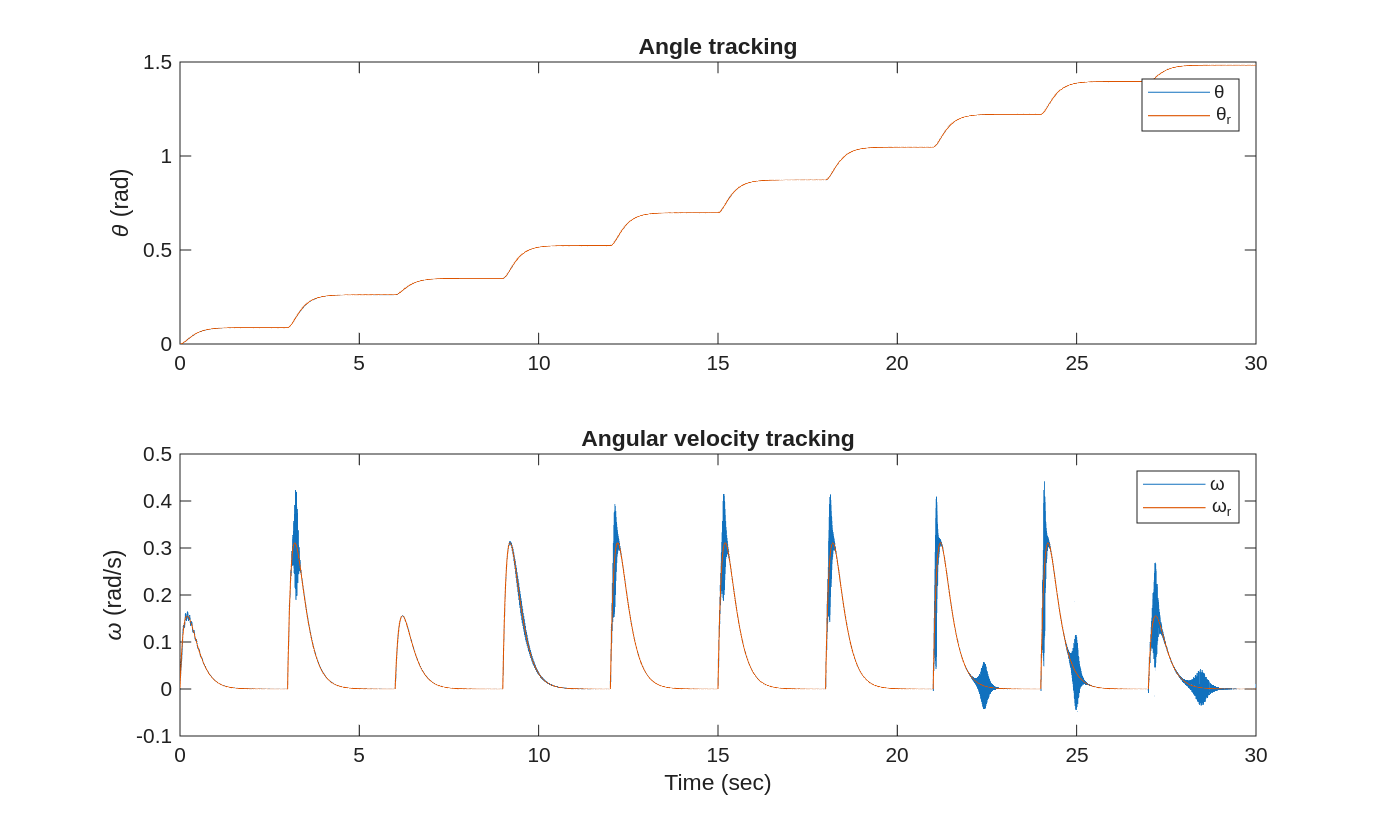
\includegraphics[width=\textwidth]{tracking-5-uncertainty.png}
            \caption{\textbf{Διάγραμμα 2.2.1.1} Διάγραμμα παρακολούθησης της γωνίας (πάνω) και της ταχύτητας (κάτω) για αβεβαιότητα ως προς τις πραγματικές τιμές των παραμέτρων του κινητήρα \(5\%\).}
        \end{subfigure}
        \begin{subfigure}{\textwidth}
            \centering
            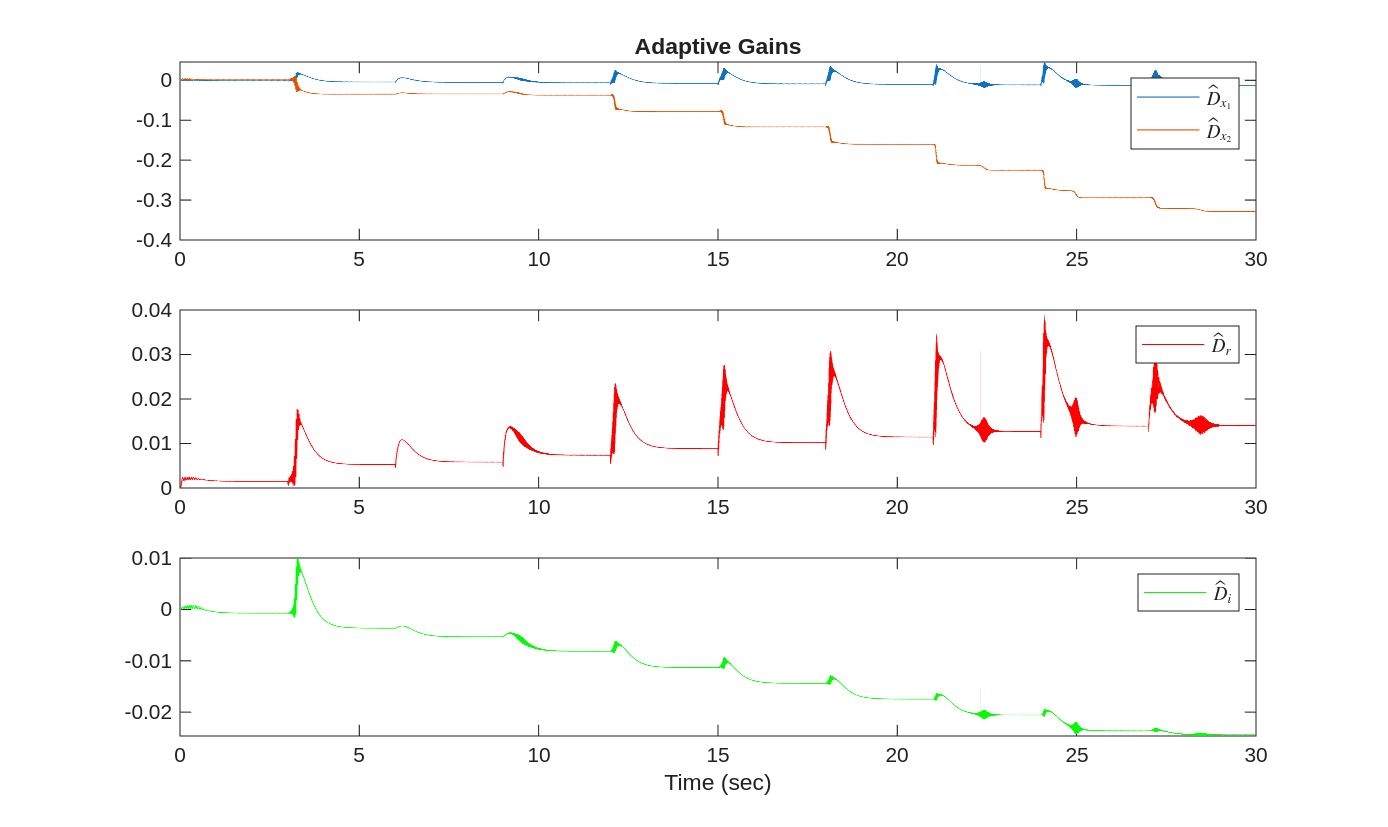
\includegraphics[width=\textwidth]{gains-5-uncertainty.png}
            \caption{\textbf{Διάγραμμα 2.2.1.2} Διαγράμματα των προσαρμοστικών κερδών του ελεγκτή για αβεβαιότητα ως προς τις πραγματικές τιμές των παραμέτρων του κινητήρα \(5\%\).}
        \end{subfigure}
    \end{figure}
    
    \subsubsection{Αβεβαιότητα \(25\%\)}
    Στην περίπτωση αυτή θα ισχύει \(a = 0.25\). Ακολουθούν τα αποτελέσματα των προσομοιώσεων.
    
    \begin{figure}[H]
        \centering
        \begin{subfigure}{\textwidth}
            \centering
            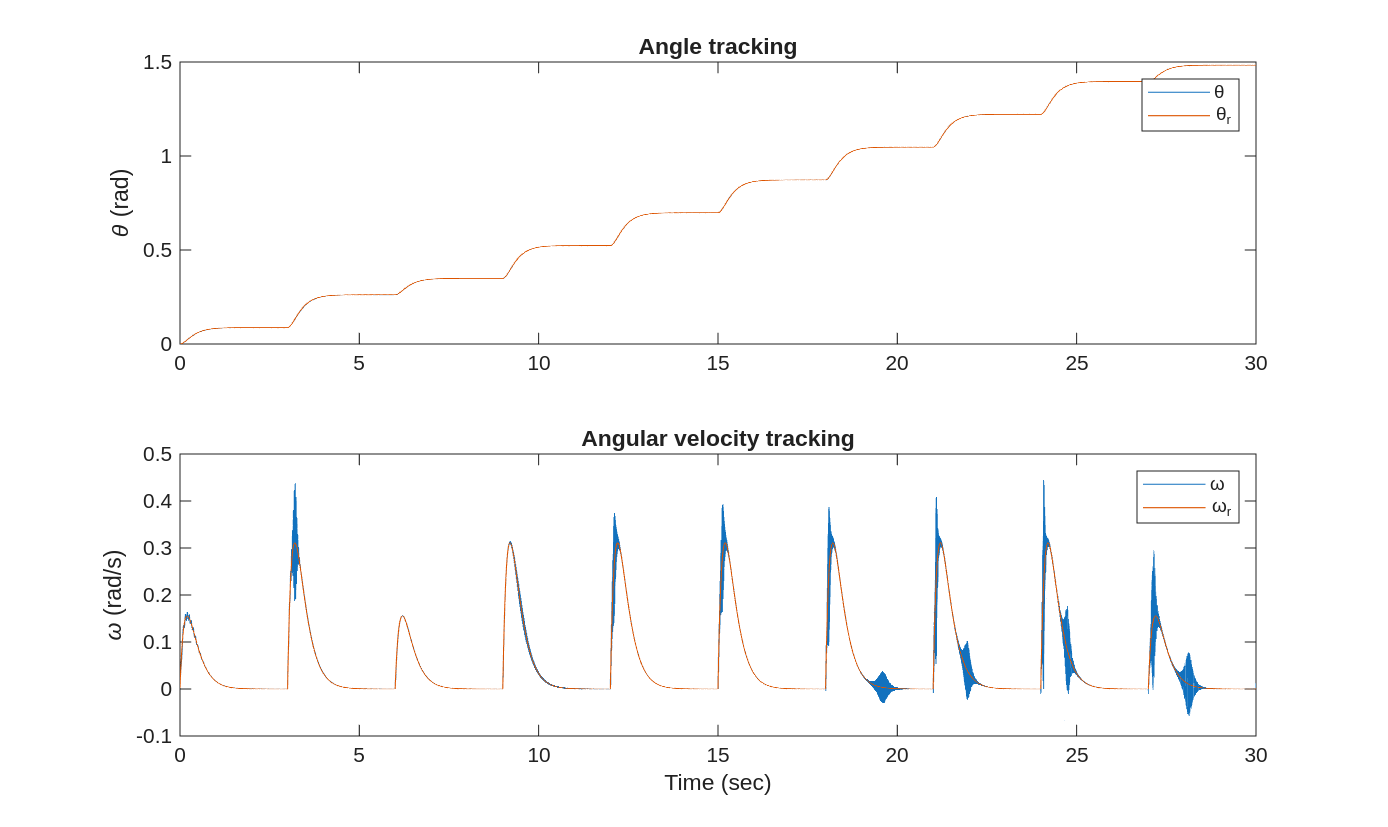
\includegraphics[width=\textwidth]{tracking-25-uncertainty.png}
            \caption{\textbf{Διάγραμμα 2.2.2.1} Διάγραμμα παρακολούθησης της γωνίας (πάνω) και της ταχύτητας (κάτω) για αβεβαιότητα ως προς τις πραγματικές τιμές των παραμέτρων του κινητήρα \(25\%\).}
        \end{subfigure}
        \begin{subfigure}{\textwidth}
            \centering
            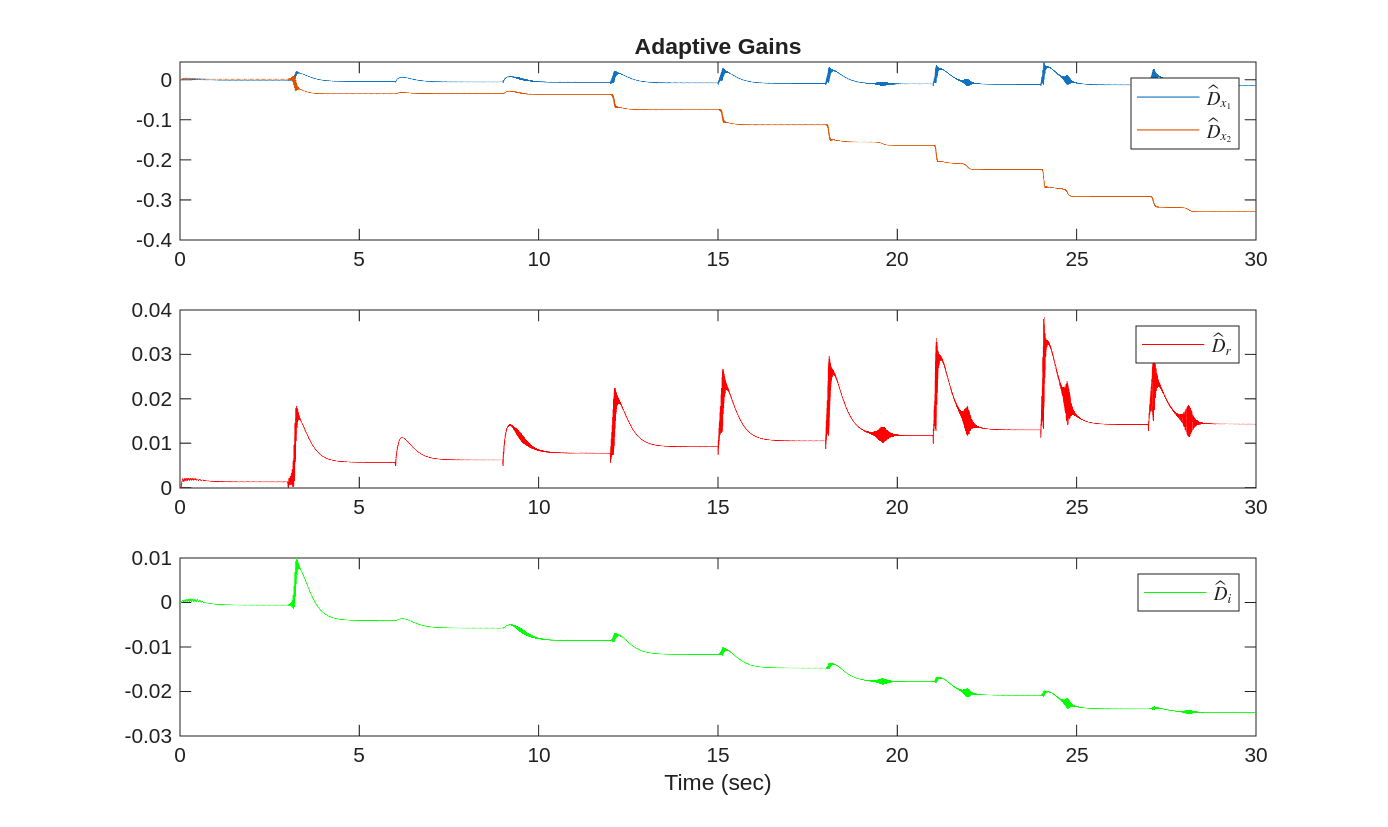
\includegraphics[width=\textwidth]{gains-25-uncertainty.png}
            \caption{\textbf{Διάγραμμα 2.2.2.2} Διαγράμματα των προσαρμοστικών κερδών του ελεγκτή για αβεβαιότητα ως προς τις πραγματικές τιμές των παραμέτρων του κινητήρα \(25\%\).}
        \end{subfigure}
    \end{figure}

    \hfill\break
    \subsubsection{Αβεβαιότητα \(50\%\)}
    Στην περίπτωση αυτή θα ισχύει \(a = 0.50\). Ακολουθούν τα αποτελέσματα των προσομοιώσεων.
    
    \begin{figure}[H]
        \centering
        \begin{subfigure}{\textwidth}
            \centering
            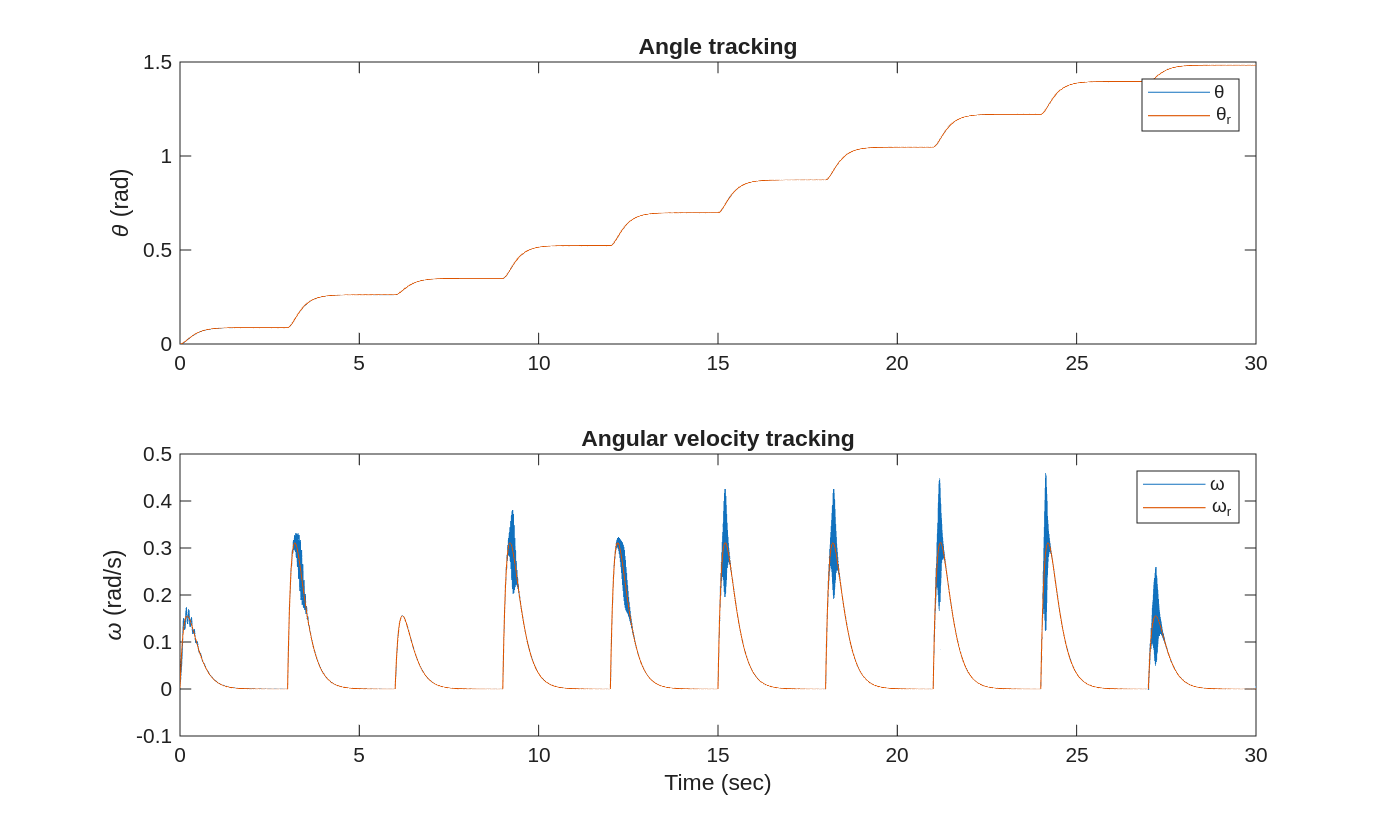
\includegraphics[width=\textwidth]{tracking-50-uncertainty.png}
            \caption{\textbf{Διάγραμμα 2.2.3.1} Διάγραμμα παρακολούθησης της γωνίας (πάνω) και της ταχύτητας (κάτω) για αβεβαιότητα ως προς τις πραγματικές τιμές των παραμέτρων του κινητήρα \(50\%\).}
        \end{subfigure}
        \begin{subfigure}{\textwidth}
            \centering
            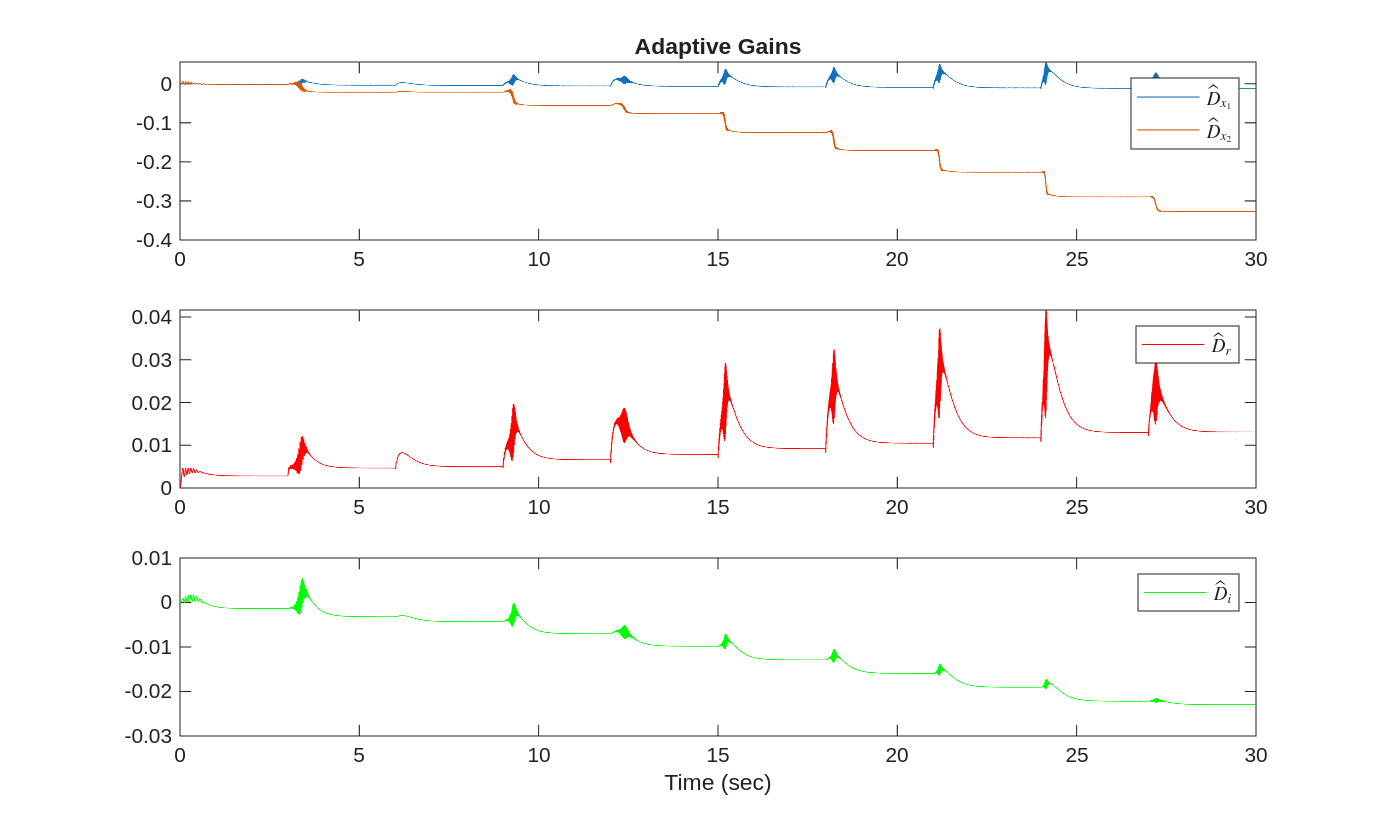
\includegraphics[width=\textwidth]{gains-50-uncertainty.png}
            \caption{\textbf{Διάγραμμα 2.2.3.2} Διαγράμματα των προσαρμοστικών κερδών του ελεγκτή για αβεβαιότητα ως προς τις πραγματικές τιμές των παραμέτρων του κινητήρα \(50\%\).}
        \end{subfigure}
    \end{figure}

    \hfill\break
    \subsubsection{Αβεβαιότητα \(75\%\)}
    Στην περίπτωση αυτή θα ισχύει \(a = 0.655\). Ακολουθούν τα αποτελέσματα των προσομοιώσεων.
    
    \begin{figure}[H]
        \centering
        \begin{subfigure}{\textwidth}
            \centering
            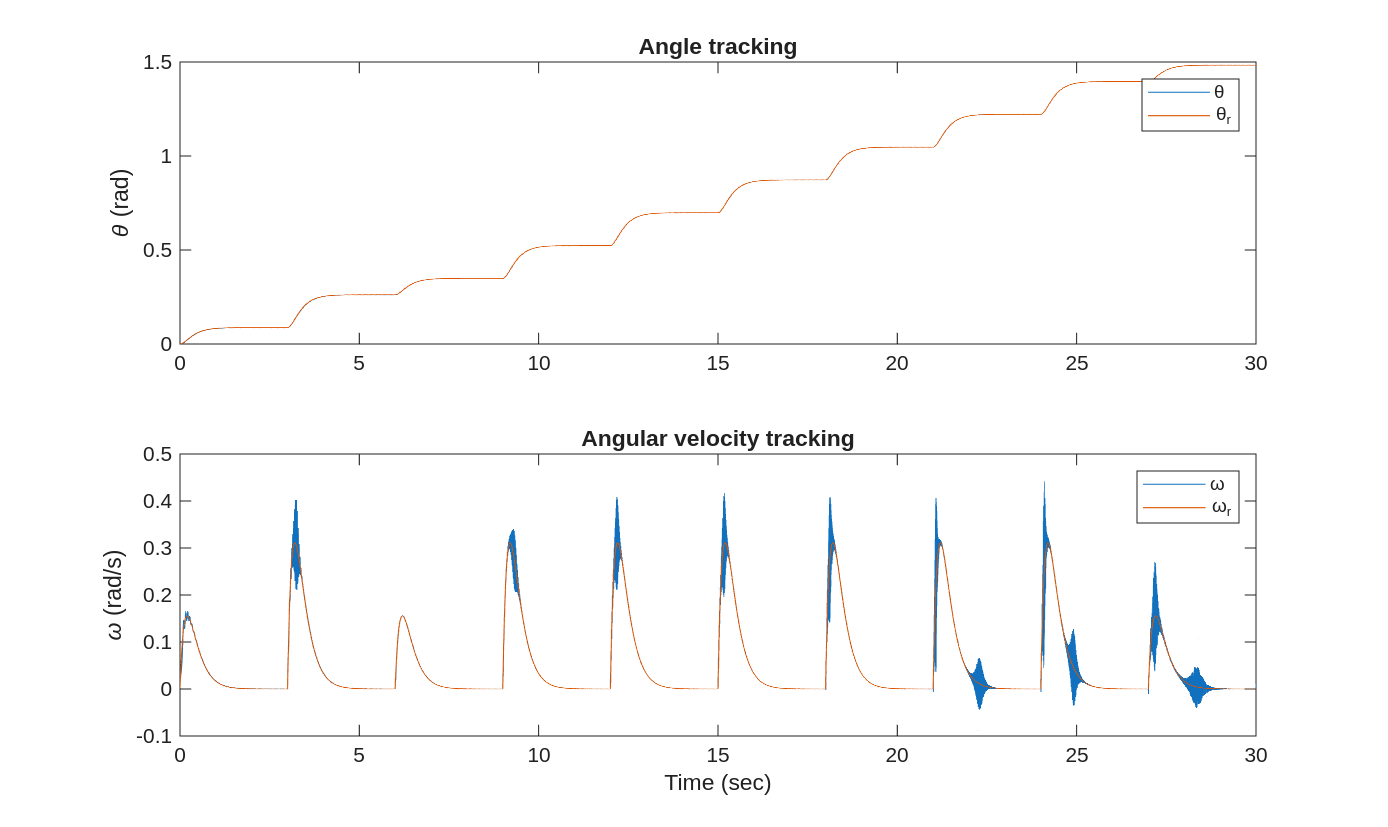
\includegraphics[width=\textwidth]{tracking-75-uncertainty.png}
            \caption{\textbf{Διάγραμμα 2.2.4.1} Διάγραμμα παρακολούθησης της γωνίας (πάνω) και της ταχύτητας (κάτω) για αβεβαιότητα ως προς τις πραγματικές τιμές των παραμέτρων του κινητήρα \(75\%\).}
        \end{subfigure}
        \begin{subfigure}{\textwidth}
            \centering
            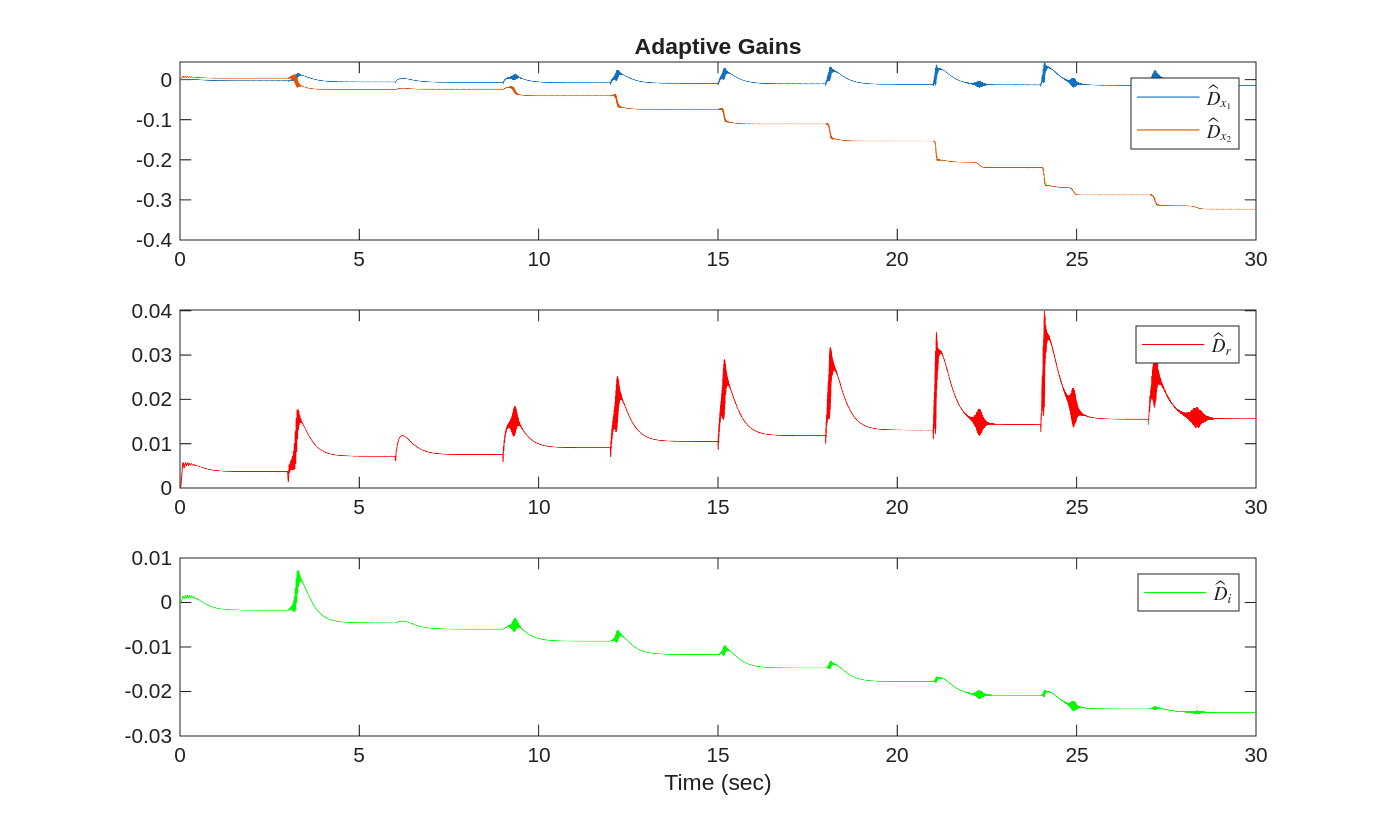
\includegraphics[width=\textwidth]{gains-75-uncertainty.png}
            \caption{\textbf{Διάγραμμα 2.2.4.2} Διαγράμματα των προσαρμοστικών κερδών του ελεγκτή για αβεβαιότητα ως προς τις πραγματικές τιμές των παραμέτρων του κινητήρα \(75\%\).}
        \end{subfigure}
    \end{figure}

    \subsection{Σχολιασμός αποτελεσμάτων για τα διάφορα επίπεδα αβεβαιότητας}
    Από τα παραπάνω διαγράμματα μπορούμε με ευκολία να παρατηρήσουμε ότι όσο η αβεβαιότητα στις πραγματικές τιμές των παραμέτρων αυξάνεται, τόσο περισσότερο το σύστημα δυσκολεύεται με την παρακολούθηση. Ειδικότερα, ενώ η γωνία ($\theta$) παρακολουθείτε σε κάθε περίπτωση ικανοποιητικά, η γωνιακή ταχύτητα ($\omega$) παρουσιάζει chattering όσο αυξάνεται η αβεβαιότητα. Αυτό οφείλεται στην προσπάθεια του προσαρμοστικού νόμου ελέγχου να αντισταθμίσει τα μεγάλα σφάλματα στη μοντελοποίηση του συστήματος. Επιπλέον, τα spikes που παρατηρούνται στα προσαρμοστικά κέρδη είναι η προσπάθεια που κάνει ο ελεγκτής να "μάθει" τις τιμές τους και γι' αυτό όσο η αβεβαιότητα αυξάνεται, η διαδικασία αυτή γίνεται ολοένα και πιο δύσκολη. Τέλος, μπορούμε να πούμε ότι ο ελεγκτής μας είναι σθεναρός, αφού το σφάλμα παρακολούθησης είναι πολύ κοντά στο μηδέν, ακόμη και στις πιο ακραίες περιπτώσεις.

    \subsection{Σύστημα παρουσία άγνωστου εξωτερικού φορτίου \(T_L(\theta)\)}
    Το μοντέλο του εξωτερικού φορτίου είναι
    \begin{equation*}
        T_L(\theta) = 10^{-3} \cdot cos(2\theta) \cdot sin(3\theta)
    \end{equation*}

    \hfill\break
    Ακολουθώντας την ίδια διαδικασία με πριν και ενσωματώνοντας το νέο δεδομένο στον ονομαστικό και τον κανονικό προσαρμοστικό νόμο ελέγχου, με αβεβαιότητα \(5\%\).

    \begin{figure}[H]
        \centering
        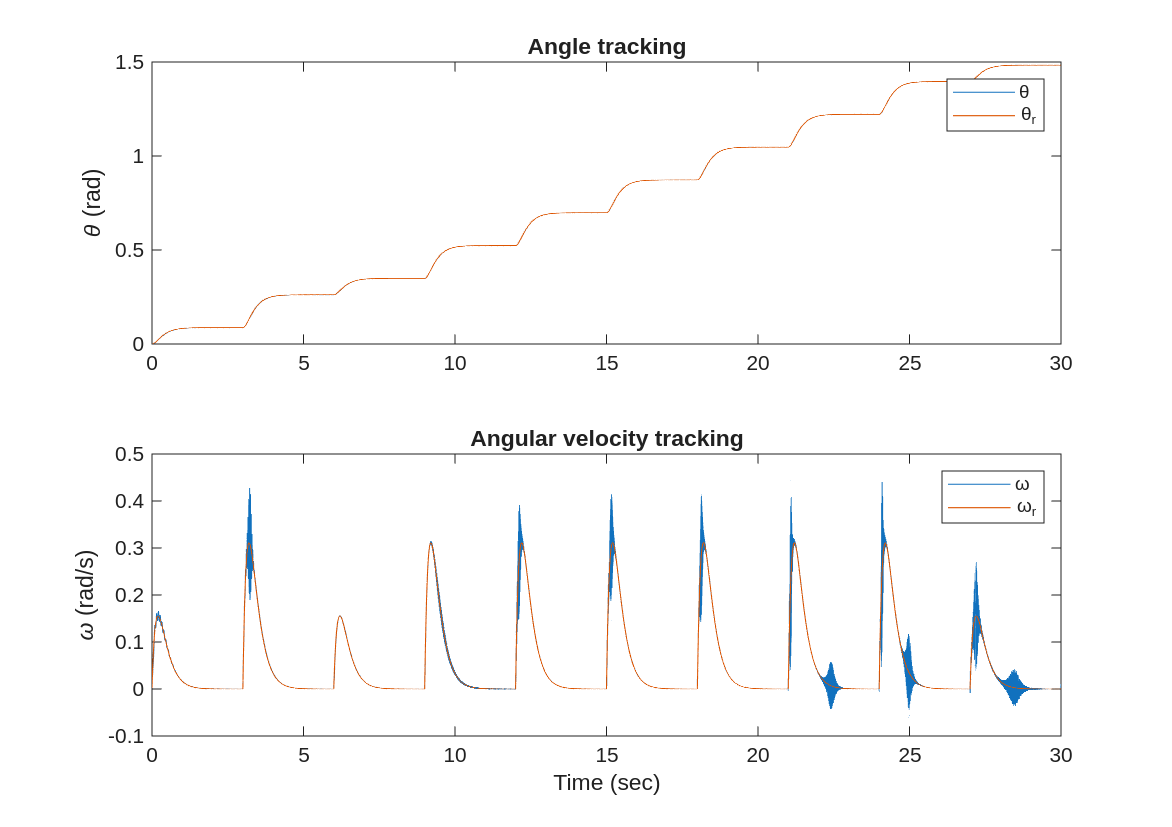
\includegraphics[width=\textwidth]{tracking-5-uncertainty-T.png}
        \caption{\textbf{Διάγραμμα 2.4.1} Διάγραμμα παρακολούθησης της γωνίας (πάνω) και της ταχύτητας (κάτω) για αβεβαιότητα ως προς τις πραγματικές τιμές των παραμέτρων του κινητήρα \(5\%\) και εξωτερικό φορτίο \(T_L(\theta)\).}
    \end{figure}
    
    \begin{figure}[H]
        \centering
        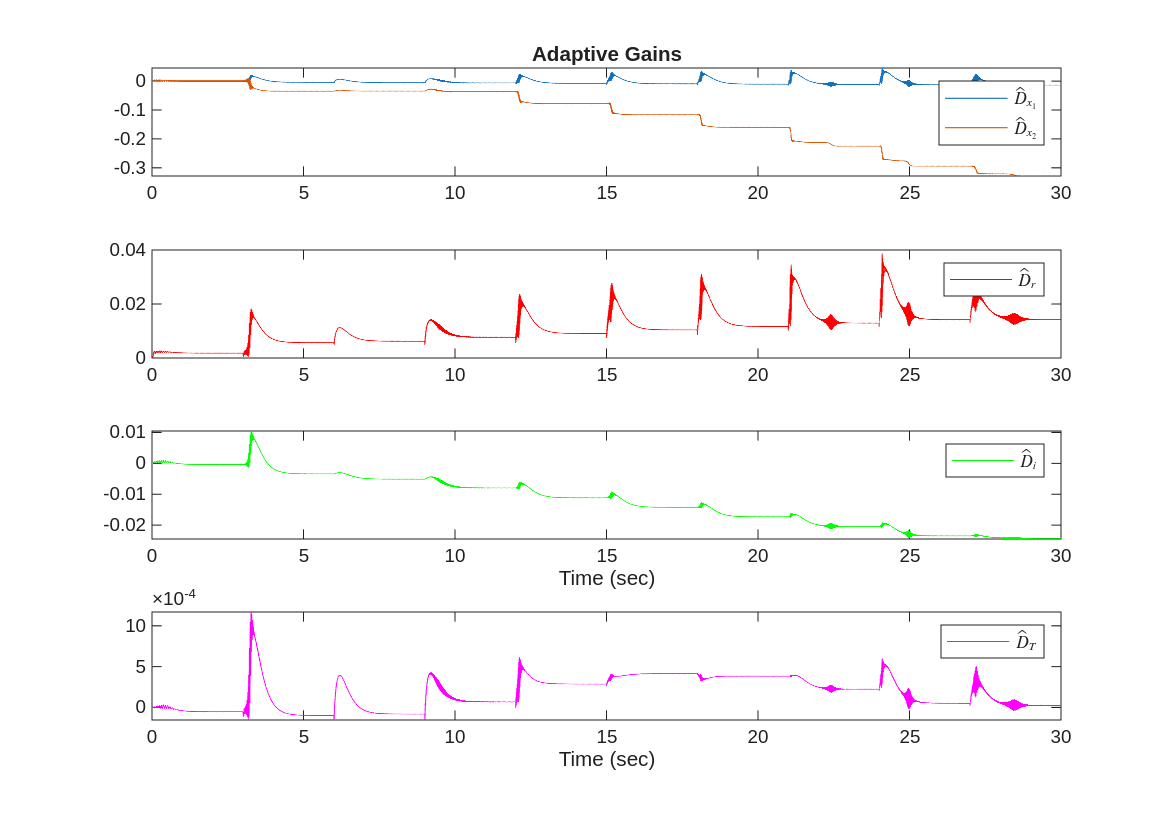
\includegraphics[width=\textwidth]{gains-5-uncertainty-T.png}
        \caption{\textbf{Διάγραμμα 2.4.2} Διαγράμματα των προσαρμοστικών κερδών του ελεγκτή για αβεβαιότητα ως προς τις πραγματικές τιμές των παραμέτρων του κινητήρα \(5\%\) και εξωτερικό φορτίο \(T_L(\theta)\).}
    \end{figure}

    \hfill\break
    Όπως μπορούμε να παρατηρήσουμε, η παρακολούθηση της γωνίας \(\theta\) γίνεται με μεγάλη ακρίβεια. Αυτό σημαίνει ότι ο ελεγκτής καταφέρνει να μάθει τις τιμές των παραμέτρων, εξαλείφοντας την αβεβαιότητα και το εξωτερικό φορτίο. Ωστόσο, η παρακολούθηση της ταχύτητας φαίνεται να εμφανίζει ξανά spikes κάθε φορά που αλλάζει η \(\theta_c\), αλλά και chattering σε ορισμένα σημεία. Όσο καλύτερα προσεγγίσουμε τις τιμές των κερδών \(\Gamma\) και όσο μικρότερες είναι, ο ελεγκτής μας δε θα αντιδρά απότομα στο να μαθαίνει τα προσαρμοστικά κέρδη. Επιπλέον, τα προσαρμοστικά κέρδη παραμένουν φραγμένα χάρη στη μέθοδο projection που χρησιμοποιήσαμε, γεγονός το οποίο μας εξασφαλίζει την ευστάθεια του συστήματος. Τέλος, μπορούμε να σχολιάσουμε ότι η απόκλιση των πραγματικών παραμέτρων ($J, K_m, B$) από τις ονομαστικές τους τιμές είναι μικρή, με αποτέλεσμα ο ελεγκτής ανταποκρίνεται άμεσα και το σύστημα συμπεριφέρεται σχεδόν σαν το ονομαστικό μοντέλο αναφοράς.
\end{document}